\documentclass[paper=a4, fontsize=11pt]{scrreprt}

\usepackage[utf8]{inputenc}
\usepackage[ngerman,english]{babel}
\usepackage{gensymb}

\usepackage[yyyymmdd]{datetime}
\renewcommand{\dateseparator}{-}

\usepackage{hyperref}

\usepackage{tikz}
\usetikzlibrary{arrows}
\usetikzlibrary{decorations.pathreplacing}

\usepackage{natbib}
\bibliographystyle{plain}

\usepackage{minted}
\usemintedstyle{rainbow_dash}

\usepackage{amsmath}
\usepackage{mathtools}

\usepackage{wrapfig}
\usepackage{multicol}
\usepackage{color}
\usepackage{pifont}

\title{Autonomous Parking Scenario}
\subtitle{Linux und L4-Mikrokern, SS 2017, Group 03}
\author{Alexander Reisner \href{mailto:alexander.reisner@tum.de}{\texttt{alexander.reisner@tum.de}} \and
Alexander Weidinger \href{mailto:alexander.weidinger@tum.de}{\texttt{alexander.weidinger@tum.de}} \and
David Werner \href{mailto:david.werner@tum.de}{\texttt{david.werner@tum.de}}}
\date{\today}

\begin{document}

% title page
\maketitle
\newpage

% toc
\tableofcontents
\newpage

% introduction
\chapter{Introduction}
This document is the final report, written by the students Alexander Reisner,
Alexander Weidinger and David Werner, for the "Linux und L4-Mikrokern" SS 2017 practical course at the Technical University of Munich.

The overall given task for the practical course was to implement an autonomous parking algorithm.

This parking algorithm is implemented as an user space application for a Pandaboard,
running the Genode OS Framework in version 16.08 with the Fiasco.OC version r56 as kernel.
We will refer to this compound as \textit{ECU} from now on.

Our ECU is integrated in the hybrid simulator framework preexisting by the KIA4SM project.
This hybrid simulator consists of a car racing simulator, Speed Dreams 2 (SD2),
a Simulation Coupler (SimCoupler), a so called \textit{S/A VM} which basically represents a multiplexing entity for each car in the simulation
and a model car representing the main car in the simulation.

Operating the model car is not part of this group's task but rather a task of the second team in this practical course.
But due to the agreed on structure of the data exchange at the Level of the ECU and S/A VM,
calculated actuator data is also received by the other team's software and can be used to control the model car.

\section{Project Overview}
Figure \ref{aw_overview} shows the overview of the project and the information flow between all involved components.
SD2 produces sensor information and sends them to the S/A VM.
The S/A VM multiplexes the data and publishes all information to the ECUs.
They are now able to compute control commands and publish them back to the S/A VM.
The S/A VM now itself receives all control commands, bundles them in a single messages
and sends them back to SD2.
This behavior runs endlessly in a loop and gets executed each simulation step.

\begin{figure}[ht]
  \begin{center}
    \begin{tikzpicture}[scale=1]
      \node[draw] at (5,0) (a){SD 2};
      \node[draw] at (5,-4) (c){S/A VM};
      \node[draw] at (0, -4) (d){ECU};
      \draw[->] (a) -- node[right] {\textit{\tiny Send sensor data}} (c);
      \draw[->, transform canvas={xshift=-0.15cm}] (c) -- node[left] {\textit{\tiny Forward actuator data}} (a);
      \draw[->, transform canvas={yshift=0.15cm}] (c) -- node[above] {\textit{\tiny Forward sensor data}} (d);
      \draw[->, transform canvas={yshift=-0.15cm}] (d) -- node[below] {\textit{\tiny Receive actuator data}} (c);
      \draw[->] (d) to [out=180,in=270,looseness=8] node [above left,xshift=-0.25cm,align=right]{\tiny\textit{Calculate next step}\\ \tiny\textit{in parking algorithm}} (d);
    \end{tikzpicture}
  \end{center}
  \caption{Overview of components}\label{aw_overview}
\end{figure}

\section{Sub Tasks}
The project was split into sub tasks, assigned to each member of the group
and also represents the parts written by each one in this report:

\begin{itemize}
  \item \textbf{Alexander Reisner}
  \begin{itemize}
    \item Design and Implementation of the S/A VM
    \item Data exchange between S/A VM and SD2
    \item Data exchange between S/A VM and ECU
    \item Implementation of the connection interface (Mosquitto client) in the ECU
    \item Final port of the Mosquitto library to the Genode OS Framework
  \end{itemize}
  \item \textbf{Alexander Weidinger}
  \begin{itemize}
    \item Extension of SD2 by a proximity sensor
    \item Data exchange between SD2 and S/A VM
    \item Extension of the human driver bot to enable autonomous driving
    \item Extend SD2 by a parked car driver bot
    \item Change starting grid of cars to allow reproducible testing results
    \item Final port of the Mosquitto library to the Genode OS Framework
  \end{itemize}
  \item \textbf{David Werner}
  \begin{itemize}
    \item Implement the autonomous parking algorithm
    \item Optimize the algorithm and adapt it for usage in our scenario
  \end{itemize}
\end{itemize}

% -------------------------
% changes to speed dreams 2
% -------------------------
\chapter{Speed Dreams 2}
Speed Dreams 2 is a fork of The Open Racing Car Simulator (TORCS)
and was used as our main car simulation.
Since the simulator was merely intended as a racing simulator,
it only provides limited functionality in case of virtual sensors.
Fortunately it can be easily expanded since the project itself is open source
and more or less sufficiently documented for such tasks.
Additionally there is a mailing list\footnote{\url{https://sourceforge.net/p/speed-dreams/mailman/}}
and an online forum\footnote{\url{https://community.speed-dreams.org/}},
where other people are willing to help in case of questions.

For our autonomous parking use case we needed to make some changes to SD2,
which affect the proximity sensor itself, the starting position of the cars
and finally changes to the driving bots.

% proximity sensor
\section{Proximity Sensor}
Since SD2 itself doesn't provide virtual proximity sensors,
we either need to implement one ourselves or we make use of related projects.
Luckily the "Simulated Car Racing Championship 2015" (SCRC) \cite{scrc2015} extends the TORCS simulator by two new sensors,
one being an "opponent" sensor, which measures the distance between the driving car and an opponent.
Furthermore there is a "focus" sensor, which measures the distance between the car and the track edge.

% reference implementation by the SCRC
\subsection{SCRC Implementation}
The problem with the given implementation is,
that the opponent sensor just measures the distance between two cars given the middle point of both cars.
For example in figure \ref{aw_scrc_impl} the distance between both cars should be relatively small,
since they are more or less next to each other.
But due to the implementation, the distance $d_1$ is over 2 meters and if they were directly next to each other,
the distance between both cars would be exactly 2 meters (given that each car has a width of 2 meters).
Therefore the distance given by this sensor can be used to get a basic idea on where other cars are
and how far they are away to oneself but are completely useless for our parking scenario.
The red dashed lines in the figure additionally shows the way how distances to objects are sorted into different sensors,
by calculating the angle between both cars and mapping it into a sensor,
since the implementation gives a 360\degree{} view by splitting in intervals of 30\degree{}.

\begin{figure}
\begin{center}
\begin{tikzpicture}[scale=1]
  % car 1
  \draw (0,0) -- (2,0) -- (2,3) -- (0,3) -- (0,0);
  \fill (1, 1.5) circle [radius=0.05];
  % car 2
  \draw (3,1) -- (5,1) -- (5,4) -- (3,4) -- (3,1);
  \fill (4, 2.5) circle [radius=0.05];
  % line between the two midpoints
  \draw (1, 1.5) -- (4, 2.5);
  % sensor lines
  \foreach \x in {0, 30, ..., 330} \draw[red, dashed] (1, 1.5) -- +(\x : 3);
  % distance bracket
  \draw[decoration={brace,mirror,raise=5pt},decorate] (1, 1.5) -- (4, 2.5) node[black,midway,yshift=-0.5cm] {\footnotesize $d_1$};
\end{tikzpicture}
\end{center}
\caption{Proximity sensor implemented by the Simulated Car Racing Championship 2015}\label{aw_scrc_impl}
\end{figure}

% our own implementation
\subsection{Our Implementation}
We simplify the virtual proximity sensor to a mere straight line,
with a given angle and position relative to the center of the car.

The opponent car can be cut down to four straight lines,
acting as the four sides of a car.

In order to now calculate the shortest distance to an opponent car,
the algorithm takes the following steps:

\begin{enumerate}
  \item Iterate over all opponent cars.
  \begin{enumerate}
    \item Calculate intersections between the straight line from the laser
    and the four straight lines from the sides of the opponent car.
    \item Iterate over all intersections.
    \begin{enumerate}
      \item Test if point of intersection is within the domain of the respective side of the car.
      \item\label{infront} Check if the intersection is 'in front' of the sensor.
    \end{enumerate}
    \item Save the potentially shortest distance to an opponent, if not already a shorter distance was found.
  \end{enumerate}
  \item Accept the shortest distance as the current value of the proximity sensor.
\end{enumerate}

Step \ref{infront} is necessary, since we are working with straight lines
and not vectors. Otherwise it could happen,
that objects on the other side of the car have to shortest distance to the sensor
and therefore are accepted as the current value of the sensor.
A mockup of our idea can be seen in figure \ref{aw_mockup}.
The distance $d_2$ would be the correct value for the proximity sensor,
indicated by the dashed blue line.

\begin{figure}[ht]
  \begin{center}
    \begin{tikzpicture}[scale=1]
      % car 1
      \draw (0,0) -- (2,0) -- (2,3) -- (0,3) -- (0,0);
      \fill (1, 1.5) circle [radius=0.05];
      % car 2
      \draw (3,1) -- (5,1) -- (5,4) -- (3,4) -- (3,1);
      \fill (4, 2.5) circle [radius=0.05];
      % sensor
      \draw[blue, dashed] (2, 1.5) -- +(0 : 4); % line
      \fill[blue] (2, 1.5) circle [radius=0.05]; % starting point
      % intersections
      \draw[blue] (3, 1.5) circle [radius=0.1];
      \draw[blue]  (5, 1.5) circle [radius=0.1];
      % distance bracket
      \draw[decoration={brace,mirror,raise=5pt},decorate] (2, 1.5) -- (3, 1.5) node[black,midway,yshift=-0.5cm] {\footnotesize $d_2$};
    \end{tikzpicture}
    \caption{Mockup of our (laser) proximity sensor implementation}\label{aw_mockup}
  \end{center}
\end{figure}

\subsubsection{Implementation}

Since a sensor position is described relative to the center point of a car,
we need to move the starting point of the sensor to the correct absolute position.
The distance from the center point to the sensor is calculated
and the x and y coordinates added to the absolute position of the car,
in regard to the yaw of the car (see listing \ref{aw_sensor_position}).

\begin{listing}[ht]
  \inputminted[firstline=91,linenos=true,lastline=96,gobble=2]{c++}{../../../simulators/speed-dreams/src/libs/sensors/obstacleSensors.cpp}
  \caption{\texttt{src/libs/sensors/obstacleSensors.cpp}}\label{aw_sensor_position}
\end{listing}

To calculate the straigt line equation $m*x+t=y$ of the sensor,
$m$ must be calculated by adding the custom angle to the current yaw of the car
and using $tan$. $t$ can be then obtained by simple inserting the x and y coordinates of the sensor.
The associated code can be seen in listing \ref{aw_mt}.

\begin{listing}[ht]
  \inputminted[firstline=105,linenos=true,lastline=104,gobble=2]{c++}{../../../simulators/speed-dreams/src/libs/sensors/obstacleSensors.cpp}
  \inputminted[firstline=110,linenos=true,lastline=109,gobble=2]{c++}{../../../simulators/speed-dreams/src/libs/sensors/obstacleSensors.cpp}
  \caption{\texttt{src/libs/sensors/obstacleSensors.cpp}}\label{aw_mt}
\end{listing}

After calculating the straight line equation for the sensor,
we need to create four additional ones, representing the four sides of the car.
We calculate the slope $m$ by using the yaw of the car, to get the left and right sides
and for the front and back sides we use the yaw + 90\degree{}.
These four straight lines are moved to the correct position,
again relative to the center of the obstacle car (compare listing \ref{aw_mt_obst}).

\begin{listing}[ht]
  \inputminted[firstline=130,linenos=true,lastline=152,gobble=3]{c++}{../../../simulators/speed-dreams/src/libs/sensors/obstacleSensors.cpp}
  \caption{\texttt{src/libs/sensors/obstacleSensors.cpp}}\label{aw_mt_obst}
\end{listing}

Now that all five straight lines are calculated,
only left is the computation of the intersections between the straight line of the sensor
and the four straight lines, representing the sides of the obstalce car (see listing \ref{aw_intersect}).

\begin{listing}[ht]
  \inputminted[firstline=154,linenos=true,lastline=164,gobble=3]{c++}{../../../simulators/speed-dreams/src/libs/sensors/obstacleSensors.cpp}
  \caption{\texttt{src/libs/sensors/obstacleSensors.cpp}}\label{aw_intersect}
\end{listing}

After obtaining the intersections, the domain is checked by verifying,
that the intersection is between the two points restricting the side of the car.
Additional to that, we need to make sure the obstacle isn't behind the sensor.
For that we reuse our \texttt{is\_between} function (which checks if a point is between two points) and adding a reference point,
which basically is an additional point 'behind' the sensor (see listing \ref{aw_ref}).

\begin{listing}[ht]
  \inputminted[firstline=98,linenos=true,lastline=99,gobble=2]{c++}{../../../simulators/speed-dreams/src/libs/sensors/obstacleSensors.cpp}
  \caption{\texttt{src/libs/sensors/obstacleSensors.cpp}}\label{aw_ref}
\end{listing}

Now that we can find the nearest intersection between a sensor and an obstacle car,
we do this in a loop for all sensors and all cars and therefore receive the correct distance value for each sensor.

\subsubsection{Usage}
As an example on how to use the newly created obstacleSensors library,
one can take a look at the human driver in listing \ref{aw_sensors}.

\begin{listing}[ht]\label{aw_sensors}
  \inputminted[firstline=245,linenos=true,lastline=256,gobble=4]{c++}{../../../simulators/speed-dreams/src/drivers/human/human.cpp}
  \caption{\texttt{src/drivers/human/human.cpp}}
\end{listing}

The code adds three sensors, one in the front with 0\degree{} angle
and one in the back with an angle of 180\degree{}.
Both sensors are moved relative to the center point of the car,
according to the schematics in the comment.
The last sensor (second sensor in the example code) is directed in an 90\degree{} angle
and moved to the right side of the rear axle.
As a side note, all three sensors have a maximum range of 20 meters,
which can be changed with the last parameter.

\subsubsection{Evaluation}
\begin{figure}
  \begin{center}
  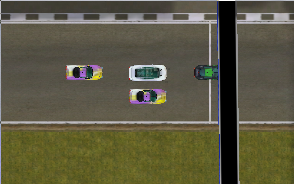
\includegraphics[scale=0.5]{aw_imgs/parked.png}
\end{center}
\caption{test}\label{aw_parked_img}
\end{figure}

Given the situation in figure \ref{aw_parked_img}
(we are the white car) and having one sensor in the front,
one in the back and one to the right,
we receive the following values for the sensors:
\begin{itemize}
  \item \textbf{Front:} 3.306382
  \item \textbf{Back:} 3.400575
  \item \textbf{Right:} 1.010126
\end{itemize}

While with the implementation by the SCRC project,
we receive different values:
\begin{itemize}
  \item \textbf{Front:} 8.086382
  \item \textbf{Back:} 8.180575
  \item \textbf{Right:} 3.010126
\end{itemize}

This means, that our sensor implementation is much more precise
and usable for the parking scenario.

\subsubsection{Open points}
Our main focus was getting the overall setup running,
therefore a few open points are still left open
and can be fixed in future versions.

The whole implementation is based on straight lines
and therefore needs some workarounds to deal with directions.
To overcome this issue it would make sense to change the implementation to vectors.
This could also fix some potential glitches with wrong distance values,
which can occur on collisions due to precision errors.
Lastly the implementation only represents a laser proximity sensor
in contrast to the implementation by the SCRC,
which can detect or more precisely assigns opponents in angle ranges.

\section{Starting Grid}
In order to test the successful execution of our parking algorithm,
we need to be able to get reproducible results in every run.

\subsection{Idea}
As we are not able to create some kind of run configuration files for SD2
and an implementation of such a system would take a lot of work,
we made use of the starting grid in the initialization phase of a race.

\subsection{Implementation}
Normally the \textit{*.xml} file of a track specifies the number of rows,
the cars are placed in at the start line.
The distance between the cars is then automatically adjusted and calculated,
taking in mind the overall width of the track, the course of the road, etc.

For the purpose of the parking scenario we hard coded the row value to one:
\begin{listing}[ht]
  \inputminted[firstline=309,linenos=true,lastline=311,gobble=1]{c++}{../../../simulators/speed-dreams/src/modules/racing/standardgame/raceinit.cpp}
  \caption{\texttt{src/modules/racing/standardgame/raceinit.cpp}}
\end{listing}

We also made sure to place each car 8 meters further away from the start line by choosing a fix value in the code.
Additionally to get the second and last car to either be 3 meters to the left or right,
we adapted the position change to the right accordingly in the code:
\begin{listing}[ht]
  \inputminted[firstline=316,linenos=true,lastline=327,gobble=4]{c++}{../../../simulators/speed-dreams/src/modules/racing/standardgame/raceinit.cpp}
  \caption{\texttt{src/modules/racing/standardgame/raceinit.cpp}}
\end{listing}

In order to ensure, that the changes don't interfere with future development,
the changes only get used, if the code is compiled with the \texttt{PARKING} option enabled.

\section{Driving bots}
Also changes were needed for two of the bots in SD2,
since although we still want to be able to drive for ourselves,
we need to make sure the car can move autonomously.
Additionally we need parked cars for our proximity sensor to detect.
We chose to make use of the \textit{human} driver and extend it by the autonomous driving
and the \textit{usr} driver to act as the parked car.

\subsection{human}
The changes to the \textit{human} bot consitsts of two parts.
First add the data exchange between SD2 and the S/A VM
and second include an autonomous driving logic.

The code for the data exchange is relatively trivial,
since its a simple socket based connection,
where SD2 acts as the server and globally listens for connections on port 9002.
The message flow between the S/A VM and SD2 is always the same
and based on an exchange between both applications.
First SD2 collects all sensor information (proximity sensors, spin velocity of the wheels, etc.)
and packs this data into a Protobuf \textit{State} message.
(For an explanation of the Protobuf message see bla) %TODO reference to AR

The Protobuf message is then serialized to a String,
the length of this message gets extracted
and both information are transmitted over the socket connection,
as can be seen in listing \ref{aw_send}.

\begin{listing}[ht]
  \inputminted[firstline=352,linenos=true,lastline=363,gobble=4]{c++}{../../../simulators/speed-dreams/src/drivers/human/human.cpp}
  \caption{\texttt{src/drivers/human/human.cpp}}\label{aw_send}
\end{listing}

For the back channel, SD2 receives a Protobuf \textit{Control} message from the S/A VM,
following the same protocol (message length, message content).
This message is parsed and information about the desired speed,
if the car will drive autonomously and the intended steering angle are interpreted.

The autonomous driving logic is simplified to accelerate with a maximum force,
if the desired speed is higher than the current speed
and to brake with maximum force if the desired speed is lower than the current speed.
This is necessary,
since the autonomous parking algorithm only is capable of providing a desired velocity
and no acceleration or deceleration commands.
The autonomous driving logic gets activated,
as soon as the \textit{Control} message sends an \texttt{autonomous=true} value.
We integrated a safety feature to always brake with full force,
if the car was driving autonomously but isn't anymore
and the driver didn't take back control until now, see listing \ref{aw_safety}.

\begin{listing}[ht]
  \inputminted[firstline=422,linenos=true,lastline=426,gobble=6]{c++}{../../../simulators/speed-dreams/src/drivers/human/human.cpp}
  \caption{\texttt{src/drivers/human/human.cpp}}\label{aw_safety}
\end{listing}

This of course only makes sense for the parking scenario
and a different approach should be taken for autonomous driving, e.g. on the highway.
A failure of an ECU while driving on the highway obviously shouldn't lead to a full brake.

\subsection{usr}
The \textit{usr} bot should be extended to just stay at the current position
and don't move in any way to represent a parked car.
We can achieve this behavior by forcing the \texttt{accelCmd} to a value of zero,
the \texttt{brakeCmd} to a value of 1 and the \texttt{steerCmd} to a value of zero,
as seen in listing \ref{aw_parked}.

\begin{listing}[ht]
  \inputminted[firstline=751,linenos=true,lastline=755,gobble=4]{c++}{../../../simulators/speed-dreams/src/drivers/usr/src/usr.cpp}
  \caption{\texttt{src/drivers/usr/src/usr.cpp}}\label{aw_parked}
\end{listing}

This solution does work quite well in our setup,
but the code should be moved to a completely new driving bot with an expressive name for the future,
to still be able to use the \textit{usr} bot in its normal programming.

\section{SimCoupler}
In the beginning of the practical course,
it was planned to interpose the Simulation Coupler (SimCoupler) between SD2 and the S/A VM.
To ease up the development process, reduce latency and
prevent additional sources of errors we decided to exclude the SimCoupler for now.
Until the end of the practical course we had to cope with latency problems,
optimization issues of the parking algorithm and other unforeseeable obstacles.
In the end we didn't have enough time to reintroduce the SimCoupler
but for the future it should be easily expendable,
since for this use case the SimCoupler more or less acts as a proxy
and doesn't introduce any additional logic.
The only problem with such an integration could be an foible of the Protobuf library,
that multiple instances of a protobuf library are tricky to integrate in a single project.
Also see a discussion of this topic on StackOverflow \cite{soprotobuf} with possible solutions.
\begin{itemize}
  \item Where do we need to make changes to integrate it
\end{itemize}
\newpage
\chapter{S/A VM}
\section{Data exchange with speedDreams 2}
  \subsection{Protobuf}
Google Protobuf is a protocol for data exchange.
The newest version can be found \href{https://github.com/google/protobuf}{here}.
To exchange data, protobuf files have to be created beforehand.
One of the protobuf files designed during this pratical course looks like this:
  \begin{figure}[!h]
  \begin{minipage}{0.5\textwidth}
  \centering
    \begin{minted}[fontsize=\tiny]{protobuf}
	syntax = "proto3";
	package protobuf;

	import "sensor.proto";
	import "wheel.proto";
	import "specification.proto";

	message State {
	  repeated Sensor sensor = 1;
	  repeated Wheel wheel = 2;
	  Specification specification = 3;
	  float steer = 4;
	  float brakeCmd = 5;
	  float accelCmd = 6;
	}
    \end{minted}
  \end{minipage}
  \begin{minipage}{0.5\textwidth}
    \begin{itemize}
\item The version of the syntax is defined.
\item All packages and imports are declared.
\item The message is constructed. Attributes can be other Protobuf messages, simple datatypes, like int or float, or a list "repeated" of any attributes named.
    \end{itemize}
  \end{minipage}
    \caption{\tiny state.proto}
  \end{figure}
  \subsection{TCP/IP} \label{tcpip}
Before any network interaction can take place, the network has to be initialized. Therefore the library lwip is usually needed. But since the mosquitto library already initializes lwip, another initialization within the components code caused lwip and moquitto to freeze.\newline
Furthermore dhcp and manuall ip configuration have to be seperated in the initialization, since dhcp ip assignement takes up to 10 seconds, however manuall ip assignement takes place instantly.
The configuration takes place in the run file of the component.\newline
\begin{figure}[!h]
  \centering
    \begin{minted}[fontsize=\tiny]{cpp}
<network dhcp="yes" ip-address="192.168.178.3" subnet-mask="255.255.255.0" default-gateway="192.168.178.1" />
<speedDreams ip-address="10.200.32.15" port="9002" />
<mosquitto ip-address="10.200.32.15" port="1883" />
    \end{minted}
    \caption{\tiny S/A VM run file}
  \end{figure}
If dhcp is set to "yes" any following configuration is ignored.\newline
If dhcp is set to "no" there is our address followed by the subnetmask and the default gateway of the VDE adapter or the connected ethernet network.\newline
SpeedDreams2's address and port as well as mosquitto server's address and port can be configured.
  \section{Our protocol} \label{ourprotocol}
To be able to exchange data, some preparation needs to be done beforehand. Since it is not usefull to send data without knowledge over its size, some kind of a protocol around the protobuf data exchange had to be designed. Therefore it was decided to send a 4 byte long value which contains the size of the following protobuf state, is sent to start the actual exchange. Any other messages are dropped.
  \subsection{Deserialization}
Once a message of given size was received it needs to be deserialized. Fortunately the method "ParseFromArray" does the job. Afterwards all received information is stored within a protobuf state. This object has automatically generated getter and setter methods, which makes it easy to access the actual data. Finally the multiplexing of the S/A VM takes place. Any data within the state object is published via mosquitto within the topic "state".
  \subsection{Serialization}
Right after the deserialization of the state message, a new message called control is created. Any information the S/A VM got from the ECU is now put into this protobuf object. Afterwards the object is serialized using SerializeToString. As mentioned in \ref{ourprotocol} before the actuall protobuf file can be sent over ethernet, its size in a seperate 4 byte message, initializes the data exchange. But finally the serialized protobuf message is sent back to speedDreams2 which can now continue with the next simualtion step.
  \subsection{Nagle's algorithm}
The goal of the \href{https://www.lifewire.com/nagle-algorithm-for-tcp-network-communication-817932}{nagle's algorithm} is to minimize the number of packets sent by the network stack. Therefore it piles up small messages. Unfortunately this approach brakes completely with the real time requirement of the S/A VM. Therefore this algorithm had to be disabled by activating the "TCP\_NODELAY" option of the lwip library.
  \subsection{Do not wait for answer of ECU}
To keep latency as low as possible the S/A VM answeres immediately after it got a state message from speedDreams2. No matter whether the S/A VM already got an update for the next step of the ECU. If the S/A VM waited for the ECU's mosquitto messages, there would be so much latency that speedDreams had to run in 1/8 realtime. For the sake of realtime the S/A VM does not care if it misses a message from the ECU. This is not a problem since the ECU does not care about the past but only about the next step. Therefore the ECU is able to correct missing instructions in the next step.
\newpage
\section{Data exchange with ECU}
  \subsubsection{MQTT}
\href{http://mqtt.org/}{MQTT} alias Message Queue Telemetry Transport is a protocol based on the publish-subscribe pattern.\newline
The publish-subscribe pattern describes a client server communication, where the server acts as a message broker and the clients subscribe and publish on topcis. The broker knows the subscriptions of clients and sends them a message if a message is published under a certain topic. Therefore network load can be taken from the clients and put to the server, since the clients only gets messages it is interessted in.
  \subsection{Subscribe}
The subscription is handled via "mosquittopp" which provides a method called "subscribe". This method needs the topic and the quality of message as input. Once a message on the given topic arrives at the server, the subscribed client is notified. This notification is handled by the callbacks \ref{callbacks} of mosquitto.
  \subsection{Publish}
The publishing is also handled via "mosquittopp" which provides another function called "publish". This method takes the topic, the message to be published and its size. The message finds its way to the server via the configuration done in the run file of the ECU. This configuration works the same way as described in TCP/IP \ref{tcpip} for the S/A VM.
  \subsection{Callbacks} \label{callbacks}
  \section{Starting the algorithm}
  \subsection{Car information}
Once the car length, the car width, the wheel radius and the maximum steering angle arrived at the ECU via pub/sub from the S/A VM, a new car information object is created. This needs to be done only once per ECU, since this static information does not change over time.
To be sure that the needed information arrived at the ECU boolean values were created that are set to true if a value arrived.
  \subsection{Compute next step}
The linker between pub/sub and the parking algorithm is the "receiveData" method. It is called once new values for the front, side and back laser, as well as the spin velocity, since the last timestamp, and the actual timestamp arrived. The topicality is handeld via boolean values, which are set to true, if a value arrived and set to false if a values was true and sent to the parking algorithm. Only full sets of data are used, for the sake of real time.
  \subsection{Publish next step}
After the computation of the parking step, the resulting actuator data is published on topic "car-control". The S/A VM and the team responsible for the actuator movement in the model car, subscribed to this topic. Consequently speedDreams2 and the model car execute the commands of the parking algorithm.
\chapter{ECU}
\chapter{Misc}
\begin{itemize}
  \item Porting of the mosquitto library % FIXME do we really want to add the mosquitto port in our documentation?
\end{itemize}

\bibliography{final-report_group3}

\end{document}
